
%(BEGIN_QUESTION)
% Copyright 2015, Tony R. Kuphaldt, released under the Creative Commons Attribution License (v 1.0)
% This means you may do almost anything with this work of mine, so long as you give me proper credit

Explain the purpose of the {\it lead/lag} unit installed in this feedforward system:

$$\includegraphics[width=15.5cm]{i01780x01.eps}$$

Hint: this control strategy is usually called {\it dynamic compensation}.

\vskip 10pt

Determine whether the lead/lag unit should be set for {\it lead} or for {\it lag} if we happen to know that the process temperature naturally responds to load changes faster than to fuel gas valve changes (i.e. a sudden decrease in feed flow causes a quicker rise in outlet temperature than a sudden increase in fuel gas flow to the burner assembly).

\vskip 20pt \vbox{\hrule \hbox{\strut \vrule{} {\bf Suggestions for Socratic discussion} \vrule} \hrule}

\begin{itemize}
\item{} Explain the significance of the ``+'' symbols next to the summer input lines.  How well would the system work if one or more of these inputs were inverting (``$-$'') rather than non-inverting?
\item{} Explain the consequence(s) of not having any dynamic compensation at all in this feedforward system.
\item{} Describe the test you would perform to determine whether or not this feedforward system required {\it lead} compensation or {\it lag} compensation, prior to introducing the lead/lag function block to the control strategy.
\item{} Explain why you suppose the load (feed flow) has a faster effect on temperature than the compensation (fuel gas flow), based on the physics of heat transfer in this process.
\item{} Explain what would happen in this process if the flow transmitter failed with a low signal.
\item{} Explain what would happen in this process if the flow transmitter failed with a high signal.
\item{} Identify what process characteristic(s) would dictate the lead/lag time ratio in the function block.
\item{} Identify what process characteristic(s) would dictate the lag time value in the function block.
\end{itemize}

\underbar{file i01780}
%(END_QUESTION)





%(BEGIN_ANSWER)

The {\it lead/lag} relay introduces an adjustable lead or an adjustable lag into the feedforward signal, the purpose being to equalize the fuel flow's lag time with the feed flow lag time.  By advancing or delaying the fuel flow response to changes in feed flow, we can make sure that the feedforward effect ``arrives'' at the process variable (outlet temperature) at just the right time to compensate for the change in feed.

%(END_ANSWER)





%(BEGIN_NOTES)

If the process responds faster to load changes than to fuel gas valve changes, the lead/lag unit should be set for {\it lead}, to help ``undo'' some of the inherent lag in the fuel gas flow response.

%INDEX% Control, strategies: feedforward with dynamic compensation (lead/lag)
%INDEX% Process: heater (fired) (generic)

%(END_NOTES)


